% \documentclass[10pt]{beamer}
\documentclass[10pt, aspectratio=169]{beamer}
\usepackage{natbib}
\usepackage{bibentry}
\usepackage{bm}
\nobibliography*


\usepackage{color, xcolor}
\definecolor{mydarkblue}{rgb}{0,0.08,0.45}
\definecolor{mydarkred}{HTML}{990000}
\definecolor{metropolisdark}{RGB}{35,35,59}

\usepackage{hyperref}
\hypersetup{
    colorlinks=true,
    citecolor=mydarkred,
    linkcolor=metropolisdark,
    urlcolor=mydarkblue
}

\usetheme[progressbar=frametitle]{metropolis}
\metroset{block=fill}
\usepackage{appendixnumberbeamer}

\usepackage[absolute,overlay]{textpos}

\usepackage{nccmath}
\usepackage{booktabs}
\usepackage[scale=2]{ccicons}

% \usepackage{pgfplots}
% \usepgfplotslibrary{dateplot}

% Math macros to be imported into main.tex

\def\xx{{\boldsymbol x}}
\def\qq{{\boldsymbol q}}
\def\dd{{\boldsymbol d}}
\def\XX{{\boldsymbol X}}
\def\YY{{\boldsymbol Y}}
\def\ZZ{{\boldsymbol Z}}
\def\aa{{\boldsymbol a}}
\def\bb{{\boldsymbol b}}
\def\rr{{\boldsymbol r}}
\def\cc{{\boldsymbol c}}
\def\qq{{\boldsymbol q}}
\def\WW{{\boldsymbol W}}
\def\KK{{\boldsymbol K}}
\def\II{{\boldsymbol I}}
\def\yy{{\boldsymbol y}}
\def\vv{{\boldsymbol v}}
\def\uu{{\boldsymbol u}}
\def\ww{{\boldsymbol w}}
\def\zz{{\boldsymbol z}}
\def\SS{{\boldsymbol S}}
\def\BB{{\boldsymbol B}}
\def\AA{{\boldsymbol A}}
\def\CC{{\boldsymbol C}}
\def\GG{{\boldsymbol G}}
\def\FF{{\boldsymbol F}}
\def\MM{{\boldsymbol M}}
\def\DD{{\boldsymbol D}}
\def\PP{{\boldsymbol P}}
\def\TT{{\boldsymbol T}}
\def\VV{{\boldsymbol V}}
\def\OO{{\boldsymbol O}}
\def\LL{{\boldsymbol L}}
\def\HH{{\boldsymbol H}}
\def\bphi{{\boldsymbol \phi}}
\def\QQ{{\boldsymbol Q}}
\def\UU{{\boldsymbol U}}
\def\HH{{\boldsymbol H}}
\def\XX{{\boldsymbol X}}
\def\Id{{\boldsymbol{I}}}
\def\bQQ{{\textcolor{blue}{\boldsymbol Q_n}}}
\def\bbQQ{{\textcolor{blue}{\boldsymbol Q_n^{(1)}}}}
\def\rQQ{{\textcolor{red}{\boldsymbol Q}}}

\def\balpha{{\boldsymbol \alpha}}
\def\bpsi{{\boldsymbol \psi}}
\def\ttheta{{\boldsymbol \theta}}
\def\LLambda{{\boldsymbol \Lambda}}
\def\SSigma{{\boldsymbol \Sigma}}

\def\eeps{{\boldsymbol \varepsilon}}
\def\eeta{{\boldsymbol \eta}}
\def\g{{g}}
\def\ee{{\boldsymbol e}}

\def\dif{\mathop{}\!\mathrm{d}}
\def\Proba{\mathbb{P}}
\def\MP{\mu_{\mathrm{MP}}}
\def\RR{{\mathbb R}}
\def\EE{{\mathbb E}\,}
\newcommand{\Econd}{\mathbf{E}}
\renewcommand{\vec}{\mathbf{vec}}
\DeclareMathOperator{\prox}{\mathbf{prox}}
\DeclareMathOperator{\tr}{tr}
\def\defas{\stackrel{\text{def}}{=}}
\DeclareMathOperator*{\dom}{dom}
\DeclareMathOperator*{\supp}{supp}
\DeclareMathOperator*{\Fix}{Fix}
\DeclareMathOperator*{\Var}{Var}
\DeclareMathOperator*{\argmin}{{arg\,min}}
\DeclareMathOperator*{\minimize}{minimize}
\DeclareMathOperator*{\diag}{\mathbf{diag}}

\newcommand{\Prto}[1]{
  { \xrightarrow[ #1 \to \infty]{\Pr }}
}

% \DeclareDocumentCommand{\Asto} {o} {
%   \IfNoValueTF {#1}
%   {\overset{\text{\rm a.s.}}{\longrightarrow}}
%   { \xrightarrow[ #1 \to \infty]{\text{\rm a.s.} }}
% }

\newcommand{\blue}{\color{blue}}

\definecolor{myblue}{HTML}{D2E4FC}
\newcommand*\mybluebox[1]{\colorbox{myblue}{\hspace{1em}#1\hspace{1em}}}

% !TEX root = non_convex_Courtney.tex

% Macros for the Non-Convex Catalyst Paper

%% !TEX root = non_convex_Courtney.tex

% Macros for the Non-Convex Catalyst Paper

%% !TEX root = non_convex_Courtney.tex

% Macros for the Non-Convex Catalyst Paper

%\input{macros}

\newcommand{\vs}{}
%\newcommand{\vs}{\vspace*{0.0cm}}
\newcommand{\cnt}{k}
\newcommand{\pr}{{\rm prox}}
\newcommand{\eg}{\emph{e.g.}}

\renewcommand\epsilon\varepsilon
%\newcommand{\dom}{\textrm{dom }} %counter
\newcommand{\smthpara}{\kappa} % the smoothing parameter 
\newcommand{\smthparacvx}{\kappa_{\text{\rm cvx}}} % the smoothing
                                % parameter  convex
\newcommand{\smthparainit}{\kappa_0} 
\newcommand{\env}{f_{\smthpara}}
 % envelope of the prox; f_\kappa(x; y) = f(x) + kappa/2 ||x-y||^2
\newcommand{\accx}{\tilde{x}} %the \acc_x \approx argmin f_{\kappa}(x;y_k)
\newcommand{\proxx}{\bar{x}} %the \proxx \approx argmin f_{\kappa}(x;
                             %x_{k-1})
\newcommand{\bproxx}{\bar{x}^{b}} %the \proxx \approx argmin f_{\kappa}(x;
                         
                            %x_{k-1})
%\newcommand{\prox}{p_{\frac{1}{\smthpara} f}} %writes prox: kappa f ->
                                %1/kappa f
% \newcommand{\prox}{\text{prox}} 
\newcommand{\weakcnx}{\rho} %weak convexity parameter
% \newcommand{\argmin}{\operatornamewithlimits{argmin}} %argmin
\newcommand{\sccnt}{i} %Outer counter for strong convexity
\newcommand{\scnx}{\mu} %Strong convexity constant
\newcommand{\smth}{L} %smooth parameter \beta->L
\newcommand{\globalcnt}{b} %global counter for complexity
\newcommand{\li}{\operatornamewithlimits{liminf}} %argmin
%\newcommand{\mtd}{\mathcal{M}} %optimization method M used as sub-routine

%% Strong Convexity w/ Estimate Sequences %%%%%%%%%%
\newcommand{\estseqpara}{\lambda} %Estimating sequence constants
\newcommand{\estseq}{\Phi} %Estimating sequence functions
\newcommand{\estseqquad}{\gamma} %Constant multiplied by the
                                %quad. term in estimating sequence
\newcommand{\estseqcenter}{\estseq^*} % center of the estimating sequence
%% General Math %%%%%%%%%%%%%%
\newcommand{\ip}[1] {\langle #1 \rangle } %inner product
\newcommand{\norm}[1] {\left \| #1 \right \|} %norm
\newcommand{\dist}{{\rm dist}} %distance
\newcommand{\R}{{\mathbb R}} %Real numbers
\newcommand{\N}{{\mathbb N}} %Natural numbers
\newcommand{\mtd}{{\mathcal M}} %Optimization method M
\newcommand{\proxi}{\text{prox}} %proximal operator
\newcommand{\Real}{{\mathbb R}} %Real numbers
\newcommand{\oR}{\overline \R} %Reals + infinity


%%%%%%%%% Theorems %%%%%%%%%%%%%
%\newtheorem{claim}{Claim}
%\newtheorem{theorem}{Theorem}[section]
%\newtheorem{proposition}[theorem]{Proposition}
%\newtheorem{lemma}[theorem]{Lemma}
%\newtheorem{defn}[theorem]{Definition}
%\newtheorem{corollary}{Corollary}[section]
%\newtheorem{pa}{Part}
%\newtheorem{subclaim}{Subclaim}
%\newtheorem{example}{Example}[section]

%%%Random stuff%%%
\newcommand{{\newalgosp}}{Basic 4WD-Catalyst~}%basic algo, with small space after the name
\newcommand{{\newalgo}}{Basic 4WD-Catalyst}%basic algo, no space
\newcommand{{\autonewalgosp}}{4WD-Catalyst~}%adaptive algo, with small space after the name , it was before 4WD-Catalyst-Automatic
\newcommand{{\autonewalgo}}{4WD-Catalyst}%adaptive algo, no space it was before 4WD-Catalyst-Automatic
\newcommand{\linesearch}{{Auto-adapt}}

\newcommand{\mylabel}[2]{#2\def\@currentlabel{#2}\label{#1}}
\newcommand{\mynote}[1]{{\bf \color{blue}{#1} }\\}


\newcommand{\vs}{}
%\newcommand{\vs}{\vspace*{0.0cm}}
\newcommand{\cnt}{k}
\newcommand{\pr}{{\rm prox}}
\newcommand{\eg}{\emph{e.g.}}

\renewcommand\epsilon\varepsilon
%\newcommand{\dom}{\textrm{dom }} %counter
\newcommand{\smthpara}{\kappa} % the smoothing parameter 
\newcommand{\smthparacvx}{\kappa_{\text{\rm cvx}}} % the smoothing
                                % parameter  convex
\newcommand{\smthparainit}{\kappa_0} 
\newcommand{\env}{f_{\smthpara}}
 % envelope of the prox; f_\kappa(x; y) = f(x) + kappa/2 ||x-y||^2
\newcommand{\accx}{\tilde{x}} %the \acc_x \approx argmin f_{\kappa}(x;y_k)
\newcommand{\proxx}{\bar{x}} %the \proxx \approx argmin f_{\kappa}(x;
                             %x_{k-1})
\newcommand{\bproxx}{\bar{x}^{b}} %the \proxx \approx argmin f_{\kappa}(x;
                         
                            %x_{k-1})
%\newcommand{\prox}{p_{\frac{1}{\smthpara} f}} %writes prox: kappa f ->
                                %1/kappa f
% \newcommand{\prox}{\text{prox}} 
\newcommand{\weakcnx}{\rho} %weak convexity parameter
% \newcommand{\argmin}{\operatornamewithlimits{argmin}} %argmin
\newcommand{\sccnt}{i} %Outer counter for strong convexity
\newcommand{\scnx}{\mu} %Strong convexity constant
\newcommand{\smth}{L} %smooth parameter \beta->L
\newcommand{\globalcnt}{b} %global counter for complexity
\newcommand{\li}{\operatornamewithlimits{liminf}} %argmin
%\newcommand{\mtd}{\mathcal{M}} %optimization method M used as sub-routine

%% Strong Convexity w/ Estimate Sequences %%%%%%%%%%
\newcommand{\estseqpara}{\lambda} %Estimating sequence constants
\newcommand{\estseq}{\Phi} %Estimating sequence functions
\newcommand{\estseqquad}{\gamma} %Constant multiplied by the
                                %quad. term in estimating sequence
\newcommand{\estseqcenter}{\estseq^*} % center of the estimating sequence
%% General Math %%%%%%%%%%%%%%
\newcommand{\ip}[1] {\langle #1 \rangle } %inner product
\newcommand{\norm}[1] {\left \| #1 \right \|} %norm
\newcommand{\dist}{{\rm dist}} %distance
\newcommand{\R}{{\mathbb R}} %Real numbers
\newcommand{\N}{{\mathbb N}} %Natural numbers
\newcommand{\mtd}{{\mathcal M}} %Optimization method M
\newcommand{\proxi}{\text{prox}} %proximal operator
\newcommand{\Real}{{\mathbb R}} %Real numbers
\newcommand{\oR}{\overline \R} %Reals + infinity


%%%%%%%%% Theorems %%%%%%%%%%%%%
%\newtheorem{claim}{Claim}
%\newtheorem{theorem}{Theorem}[section]
%\newtheorem{proposition}[theorem]{Proposition}
%\newtheorem{lemma}[theorem]{Lemma}
%\newtheorem{defn}[theorem]{Definition}
%\newtheorem{corollary}{Corollary}[section]
%\newtheorem{pa}{Part}
%\newtheorem{subclaim}{Subclaim}
%\newtheorem{example}{Example}[section]

%%%Random stuff%%%
\newcommand{{\newalgosp}}{Basic 4WD-Catalyst~}%basic algo, with small space after the name
\newcommand{{\newalgo}}{Basic 4WD-Catalyst}%basic algo, no space
\newcommand{{\autonewalgosp}}{4WD-Catalyst~}%adaptive algo, with small space after the name , it was before 4WD-Catalyst-Automatic
\newcommand{{\autonewalgo}}{4WD-Catalyst}%adaptive algo, no space it was before 4WD-Catalyst-Automatic
\newcommand{\linesearch}{{Auto-adapt}}

\newcommand{\mylabel}[2]{#2\def\@currentlabel{#2}\label{#1}}
\newcommand{\mynote}[1]{{\bf \color{blue}{#1} }\\}


\newcommand{\vs}{}
%\newcommand{\vs}{\vspace*{0.0cm}}
\newcommand{\cnt}{k}
\newcommand{\pr}{{\rm prox}}
\newcommand{\eg}{\emph{e.g.}}

\renewcommand\epsilon\varepsilon
%\newcommand{\dom}{\textrm{dom }} %counter
\newcommand{\smthpara}{\kappa} % the smoothing parameter 
\newcommand{\smthparacvx}{\kappa_{\text{\rm cvx}}} % the smoothing
                                % parameter  convex
\newcommand{\smthparainit}{\kappa_0} 
\newcommand{\env}{f_{\smthpara}}
 % envelope of the prox; f_\kappa(x; y) = f(x) + kappa/2 ||x-y||^2
\newcommand{\accx}{\tilde{x}} %the \acc_x \approx argmin f_{\kappa}(x;y_k)
\newcommand{\proxx}{\bar{x}} %the \proxx \approx argmin f_{\kappa}(x;
                             %x_{k-1})
\newcommand{\bproxx}{\bar{x}^{b}} %the \proxx \approx argmin f_{\kappa}(x;
                         
                            %x_{k-1})
%\newcommand{\prox}{p_{\frac{1}{\smthpara} f}} %writes prox: kappa f ->
                                %1/kappa f
% \newcommand{\prox}{\text{prox}} 
\newcommand{\weakcnx}{\rho} %weak convexity parameter
% \newcommand{\argmin}{\operatornamewithlimits{argmin}} %argmin
\newcommand{\sccnt}{i} %Outer counter for strong convexity
\newcommand{\scnx}{\mu} %Strong convexity constant
\newcommand{\smth}{L} %smooth parameter \beta->L
\newcommand{\globalcnt}{b} %global counter for complexity
\newcommand{\li}{\operatornamewithlimits{liminf}} %argmin
%\newcommand{\mtd}{\mathcal{M}} %optimization method M used as sub-routine

%% Strong Convexity w/ Estimate Sequences %%%%%%%%%%
\newcommand{\estseqpara}{\lambda} %Estimating sequence constants
\newcommand{\estseq}{\Phi} %Estimating sequence functions
\newcommand{\estseqquad}{\gamma} %Constant multiplied by the
                                %quad. term in estimating sequence
\newcommand{\estseqcenter}{\estseq^*} % center of the estimating sequence
%% General Math %%%%%%%%%%%%%%
\newcommand{\ip}[1] {\langle #1 \rangle } %inner product
\newcommand{\norm}[1] {\left \| #1 \right \|} %norm
\newcommand{\dist}{{\rm dist}} %distance
\newcommand{\R}{{\mathbb R}} %Real numbers
\newcommand{\N}{{\mathbb N}} %Natural numbers
\newcommand{\mtd}{{\mathcal M}} %Optimization method M
\newcommand{\proxi}{\text{prox}} %proximal operator
\newcommand{\Real}{{\mathbb R}} %Real numbers
\newcommand{\oR}{\overline \R} %Reals + infinity


%%%%%%%%% Theorems %%%%%%%%%%%%%
%\newtheorem{claim}{Claim}
%\newtheorem{theorem}{Theorem}[section]
%\newtheorem{proposition}[theorem]{Proposition}
%\newtheorem{lemma}[theorem]{Lemma}
%\newtheorem{defn}[theorem]{Definition}
%\newtheorem{corollary}{Corollary}[section]
%\newtheorem{pa}{Part}
%\newtheorem{subclaim}{Subclaim}
%\newtheorem{example}{Example}[section]

%%%Random stuff%%%
\newcommand{{\newalgosp}}{Basic 4WD-Catalyst~}%basic algo, with small space after the name
\newcommand{{\newalgo}}{Basic 4WD-Catalyst}%basic algo, no space
\newcommand{{\autonewalgosp}}{4WD-Catalyst~}%adaptive algo, with small space after the name , it was before 4WD-Catalyst-Automatic
\newcommand{{\autonewalgo}}{4WD-Catalyst}%adaptive algo, no space it was before 4WD-Catalyst-Automatic
\newcommand{\linesearch}{{Auto-adapt}}

\newcommand{\mylabel}[2]{#2\def\@currentlabel{#2}\label{#1}}
\newcommand{\mynote}[1]{{\bf \color{blue}{#1} }\\}

\usepackage{minted}
\usepackage[version=4]{mhchem}

\usepackage{tikz}
\usetikzlibrary{shadows,calc,backgrounds,matrix,fit}



% code adapted from https://tex.stackexchange.com/a/11483/3954

% some parameters for customization
\def\shadowshift{3pt,-3pt}
\def\shadowradius{6pt}

\colorlet{innercolor}{black!60}
\colorlet{outercolor}{gray!05}

% this draws a shadow under a rectangle node
\newcommand\drawshadow[1]{
    \begin{pgfonlayer}{shadow}
        \shade[outercolor,inner color=innercolor,outer color=outercolor] ($(#1.south west)+(\shadowshift)+(\shadowradius/2,\shadowradius/2)$) circle (\shadowradius);
        \shade[outercolor,inner color=innercolor,outer color=outercolor] ($(#1.north west)+(\shadowshift)+(\shadowradius/2,-\shadowradius/2)$) circle (\shadowradius);
        \shade[outercolor,inner color=innercolor,outer color=outercolor] ($(#1.south east)+(\shadowshift)+(-\shadowradius/2,\shadowradius/2)$) circle (\shadowradius);
        \shade[outercolor,inner color=innercolor,outer color=outercolor] ($(#1.north east)+(\shadowshift)+(-\shadowradius/2,-\shadowradius/2)$) circle (\shadowradius);
        \shade[top color=innercolor,bottom color=outercolor] ($(#1.south west)+(\shadowshift)+(\shadowradius/2,-\shadowradius/2)$) rectangle ($(#1.south east)+(\shadowshift)+(-\shadowradius/2,\shadowradius/2)$);
        \shade[left color=innercolor,right color=outercolor] ($(#1.south east)+(\shadowshift)+(-\shadowradius/2,\shadowradius/2)$) rectangle ($(#1.north east)+(\shadowshift)+(\shadowradius/2,-\shadowradius/2)$);
        \shade[bottom color=innercolor,top color=outercolor] ($(#1.north west)+(\shadowshift)+(\shadowradius/2,-\shadowradius/2)$) rectangle ($(#1.north east)+(\shadowshift)+(-\shadowradius/2,\shadowradius/2)$);
        \shade[outercolor,right color=innercolor,left color=outercolor] ($(#1.south west)+(\shadowshift)+(-\shadowradius/2,\shadowradius/2)$) rectangle ($(#1.north west)+(\shadowshift)+(\shadowradius/2,-\shadowradius/2)$);
        \filldraw ($(#1.south west)+(\shadowshift)+(\shadowradius/2,\shadowradius/2)$) rectangle ($(#1.north east)+(\shadowshift)-(\shadowradius/2,\shadowradius/2)$);
    \end{pgfonlayer}
}

% create a shadow layer, so that we don't need to worry about overdrawing other things
\pgfdeclarelayer{shadow} 
\pgfsetlayers{shadow,main}

\newsavebox\mybox
\newlength\mylen

\newcommand\shadowimage[2][]{%
\setbox0=\hbox{\includegraphics[#1]{#2}}
\setlength\mylen{\wd0}
\ifnum\mylen<\ht0
\setlength\mylen{\ht0}
\fi
\divide \mylen by 120
\def\shadowshift{\mylen,-\mylen}
\def\shadowradius{\the\dimexpr\mylen+\mylen+\mylen\relax}
\begin{tikzpicture}
\node[anchor=south west,inner sep=0] (image) at (0,0) {\includegraphics[#1]{#2}};
\drawshadow{image}
\end{tikzpicture}}

\usepackage{xspace}
\newcommand{\themename}{\textbf{\textsc{metropolis}}\xspace}

\definecolor{myorange}{RGB}{217,95,2}

\newcommand{\bbeta}{\bm{\beta}}

\title{Random Matrix Theory for Machine Learning}
\subtitle{The Mystery of Generalization: Why Does Deep Learning Work?}
% \date{\today}
\date{}
\author{Fabian Pedregosa, Courtney Paquette, Tom Trogdon, \underline{Jeffrey Pennington}}
\institute{\url{https://random-matrix-learning.github.io}}
% \titlegraphic{\hfill\includegraphics[height=1.5cm]{logo.pdf}}

\begin{document}

\maketitle




% \begin{frame}{Table of contents}
%   \setbeamertemplate{section in toc}[sections numbered]
%   \tableofcontents%[hideallsubsections]
% \end{frame}
\begin{frame}[t]{Why does deep learning work?}
Deep neural networks define a flexible and expressive class of functions.
\begin{columns}
\begin{column}{0.5\linewidth}
State-of-the-art models have millions or billions of parameters
\begin{itemize}
    \item Meena: 2.6 billion
    \item Turing NLG: 17 billion
    \item GPT-3: 175 billion
\end{itemize}
\end{column}
% \pause
\begin{column}{0.4\linewidth}
\begin{center}
    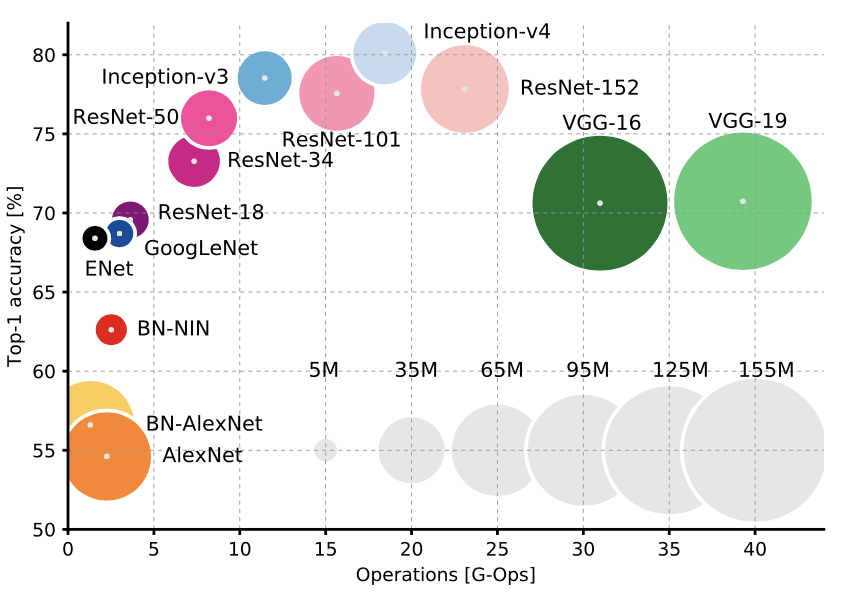
\includegraphics[width=0.75\linewidth]{part-4-images/image-model-scaling.png}
        
\vspace{-0.2cm}
{\scriptsize Source: \citep{canziani2016analysis}}
\end{center}
\end{column}
\end{columns}
\pause
\begin{columns}
\begin{column}{0.5\linewidth}
Models that perform well on real data can easily memorize noise% (Zhang et al., 2016)
\vspace{0.4cm}
\end{column}
\begin{column}{0.4\linewidth}
\begin{center}
    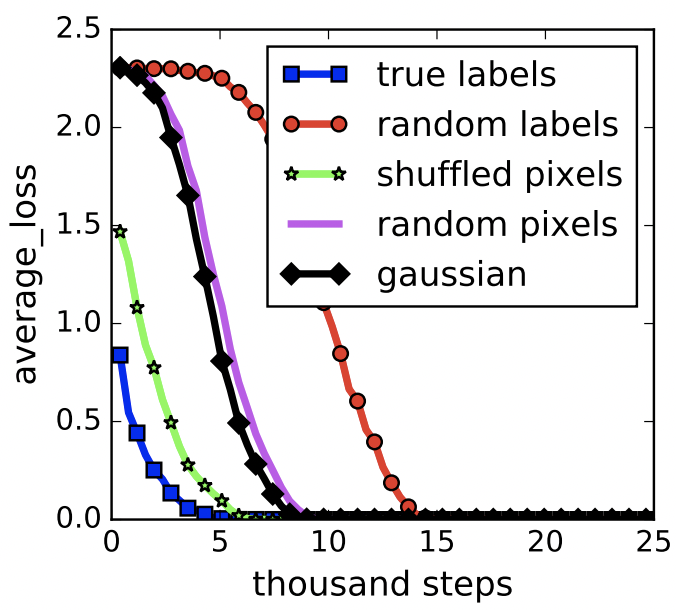
\includegraphics[width=0.55\linewidth]{part-4-images/random-labels.png} 
        
\vspace{-0.2cm}
{\scriptsize Source: \citep{zhang2021understanding}}
\end{center}
\end{column}
\end{columns}
\end{frame}
\begin{frame}[t]{Why does deep learning work?}
Deep neural networks define a flexible and expressive class of functions.
\begin{itemize}
    \item[$\Rightarrow$] Standard wisdom suggests they should overfit 
\end{itemize}
\begin{center}
    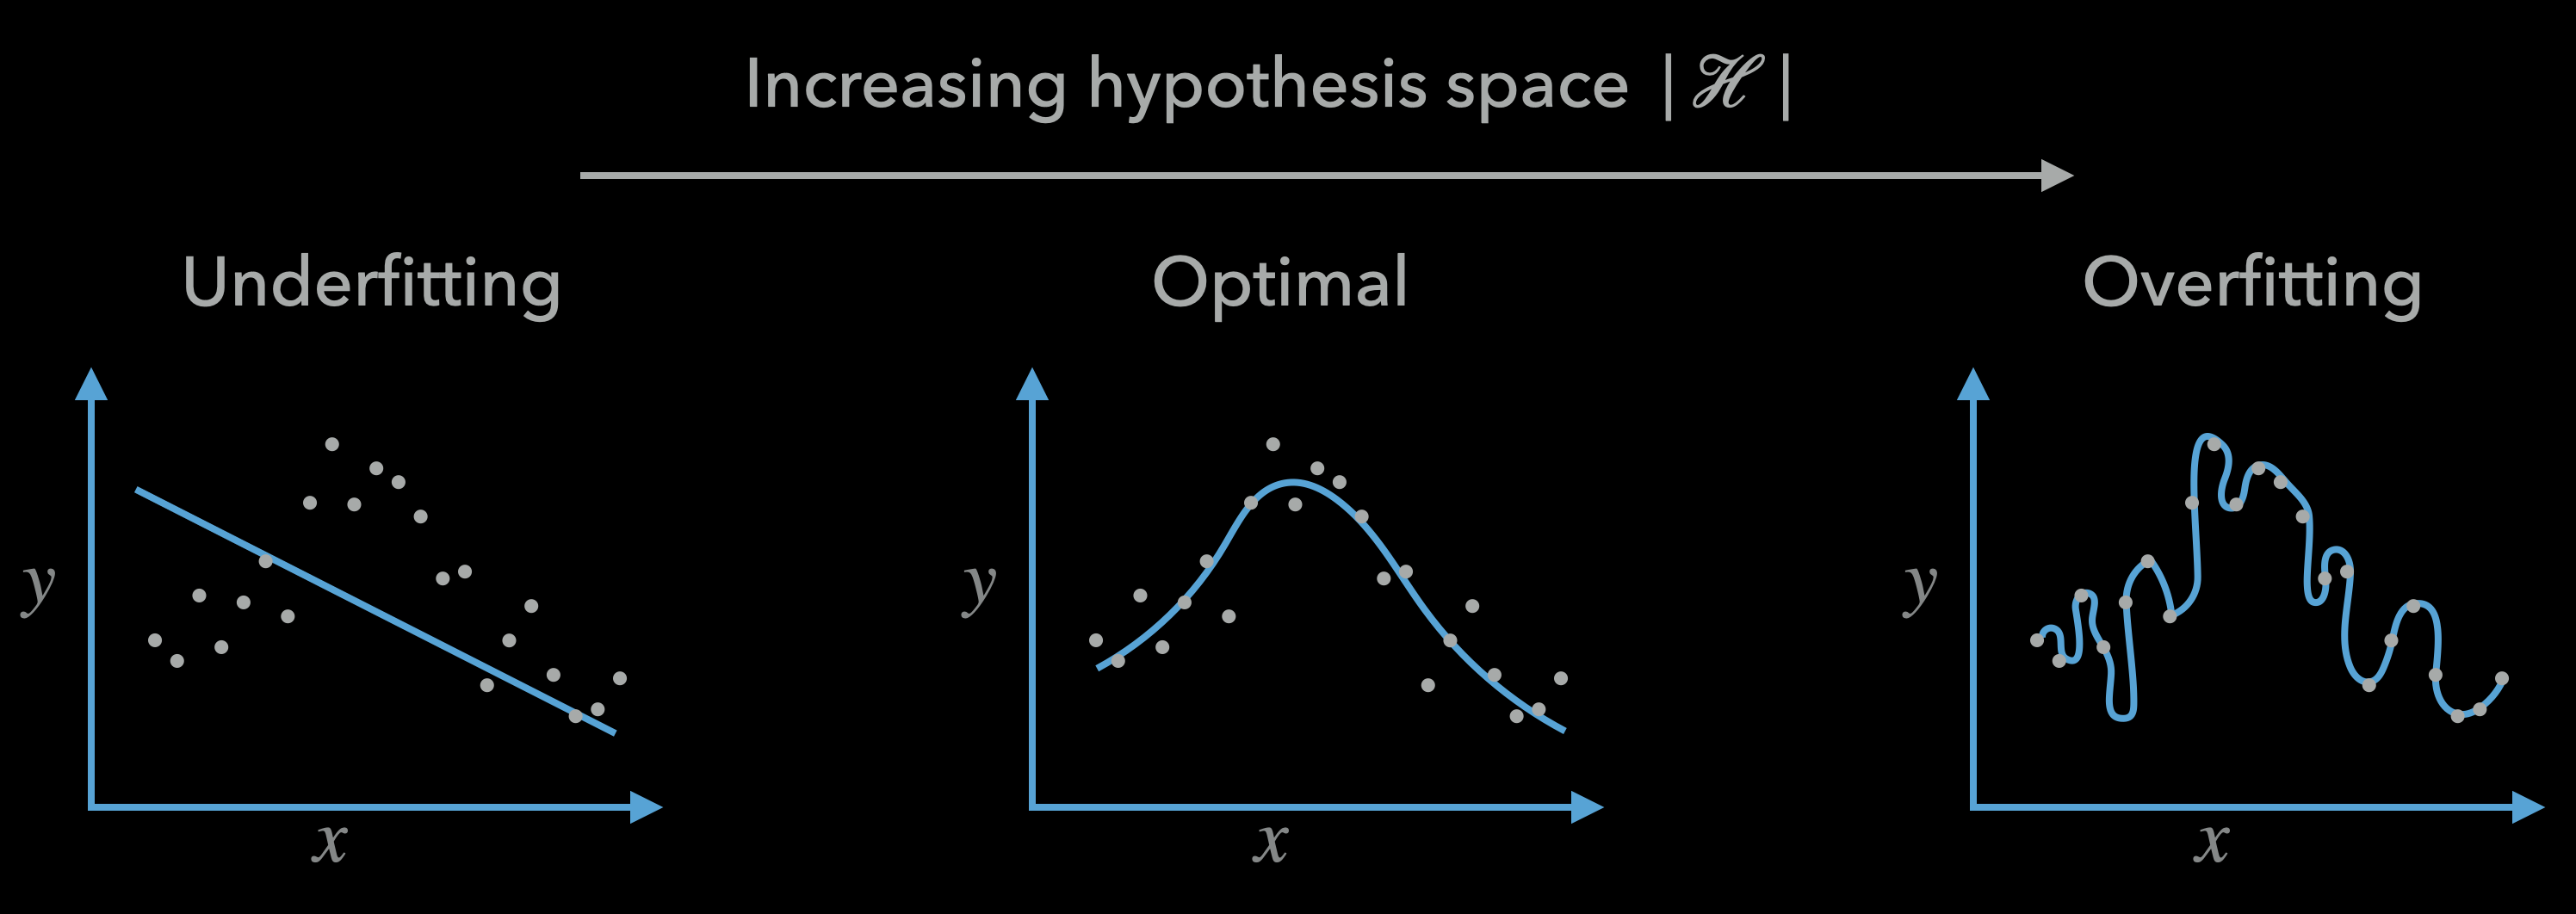
\includegraphics[width=\linewidth]{part-4-images/overfitting.png} 
\end{center}
\end{frame}
\begin{frame}[t]{Why does deep learning work?}
Deep neural networks define a flexible and expressive class of functions.
\begin{itemize}
    \item[$\Rightarrow$] Standard wisdom suggests they should overfit 
\end{itemize}
\begin{center}
    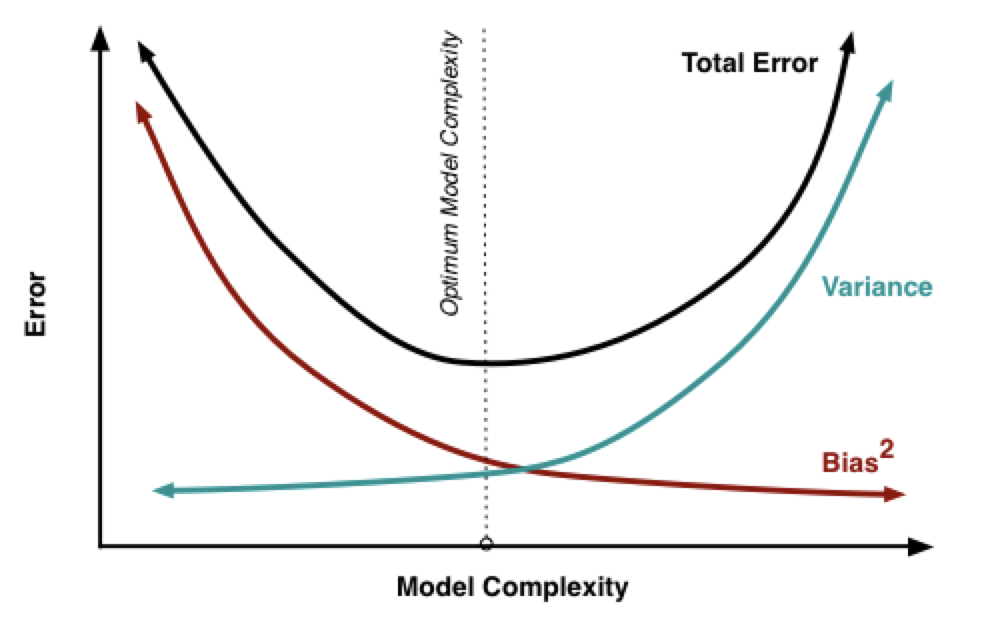
\includegraphics[width=0.6\linewidth]{part-4-images/U-curve.png} 
\end{center}
\end{frame}
%
\begin{frame}[t]{Double descent}
However, large neural networks do not obey the classical theory:
\begin{columns}
\begin{column}{0.5\linewidth}
\begin{center}
    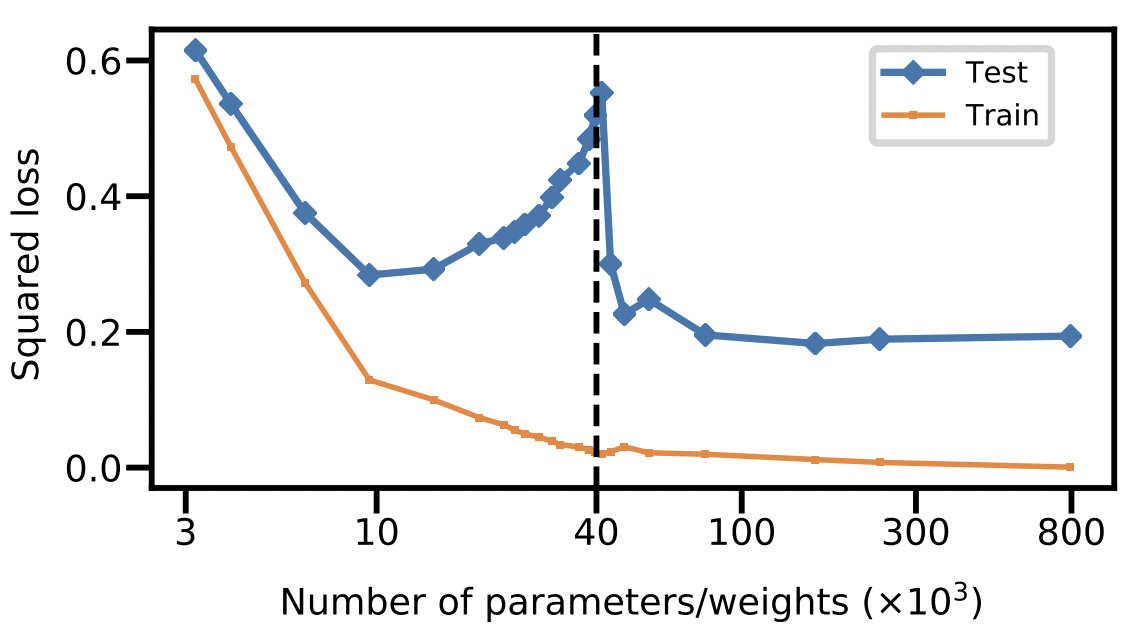
\includegraphics[width=0.5\linewidth]{part-4-images/belkin2018.png} 
        
\vspace{-0.2cm}
{\scriptsize Source: \citep{belkin2019reconciling}}
\end{center}
\begin{center}
    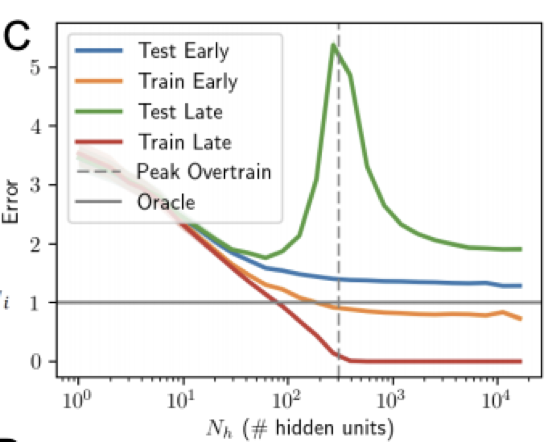
\includegraphics[width=0.5\linewidth]{part-4-images/advani.png}
    
\vspace{-0.2cm}
{\scriptsize Source: \citep{advani2020high}}
    
\end{center}
\end{column}
\begin{column}{0.5\linewidth}
\begin{center}
\hspace{-1cm}
    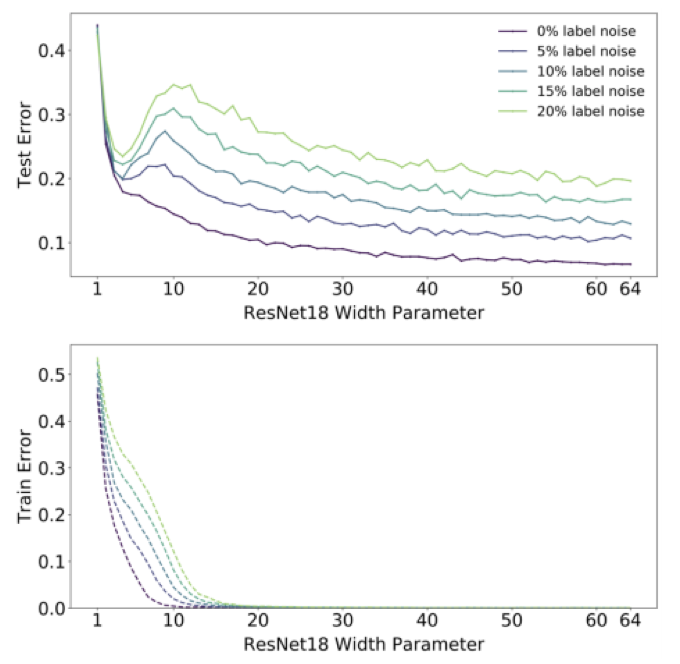
\includegraphics[width=0.75\linewidth]{part-4-images/nakkiran.png}
    
\vspace{-0.2cm}
{\scriptsize Source: \citep{nakkiran2019deep}}
\end{center}
\end{column}
\end{columns}
\vspace{0.2cm}
The emerging paradigm of \emph{double descent} seeks to explain this phenomenon.
\end{frame}
%
\section{Models of Double Descent}
\begin{frame}{History of double descent: Kernel interpolation}
1) Interpolating kernels (trained to zero error) generalize well~\citep{belkin2018understand}
\begin{itemize}
    \item[$\Rightarrow$] Double descent is not unique to deep neural\\ networks
\end{itemize}
\pause
\begin{columns}
\begin{column}{0.5\linewidth}
\hspace{0.4cm}2) Kernels can implicitly regularize in high\\\qquad\, dimensions~\citep{liang2020just}
\end{column}
\begin{column}{0.5\linewidth}
\begin{center}
\vspace{-0.6cm}
\hspace{1cm}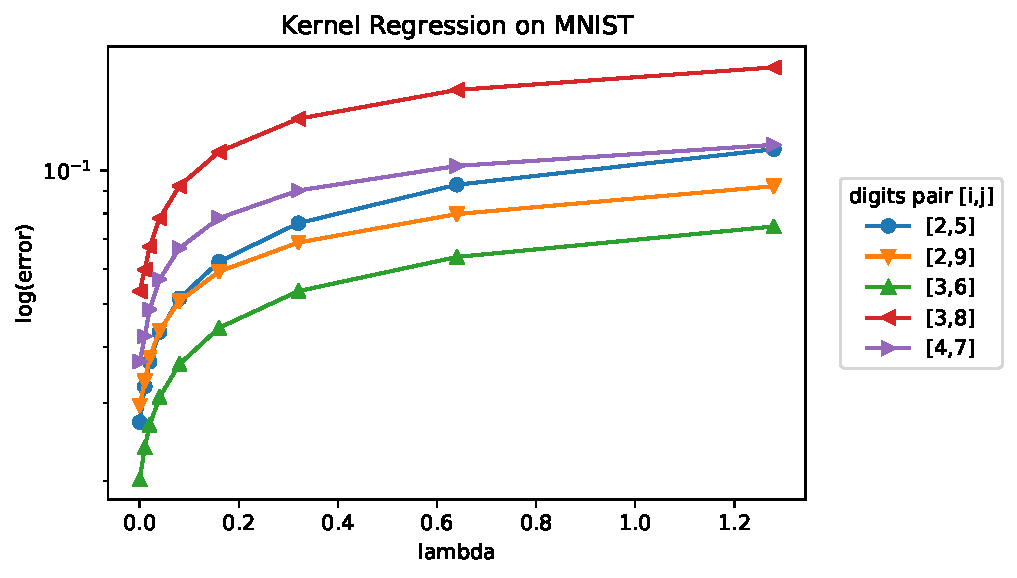
\includegraphics[width=0.8\linewidth]{part-4-images/mnist-intro.pdf}

\vspace{-0.2cm}
\hspace{1.5cm}
{\scriptsize Source: \citep{liang2020just}}
\end{center}
\end{column}
\end{columns}
\pause
% \vspace{0.0cm}
3) Consistency is a high-dimensional phenomenon~\citep{rakhlin2019consistency}:

\qquad The estimation error of the minimum-norm kernel interpolant
$$\argmin_{f\in\mathcal{H}}\; \|f\|_\mathcal{H}\quad \text{s.t.} \quad  f(x_i) = y_i\,, \;\; i=1\ldots n$$
\qquad does not converge to zero as $n$ grows, unless $d$ is proportional to $n$.
% \begin{itemize}
%     \item Empirical evidence that interpolators generalize (Belkin/Ma/Mandal)
%     \item Kernels can implicitly regularize in high dimensions (Liang and Rakhlin)
%     \item Consistency is high-dimensional phenomenon (Rakhlin and Zhai)
% \end{itemize}
\end{frame}
\begin{frame}[t]{Models of double descent: High-dimensional linear regression}
What is the simplest theoretically tractable model that exhibits double descent?
\pause

Linear regression suffices, but requires a mechanism to vary the effective number of parameters or samples:
\begin{itemize}
    \item The size of randomly selected subsets of features~\citep{belkin2020two}
    \item The dimensionality of the low-variance subspace~\citep{bartlett2020benign}
    \item The sparsity of the generative model~\citep{mitra2019understanding}
    % \item Hastie, asymptotic min-norm 
\end{itemize}
\begin{columns}
\begin{column}{0.6\linewidth}
\begin{center}
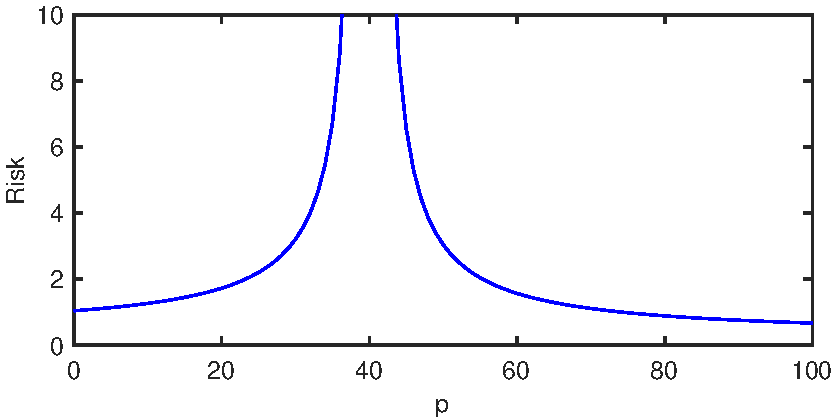
\includegraphics[width=0.7\linewidth]{part-4-images/riskplot-new.pdf}

\vspace{-0.2cm}
{\scriptsize Source: \citep{belkin2020two}}
\end{center}

\end{column}
\begin{column}{0.4\linewidth}
\begin{center}
\hspace{-1cm}
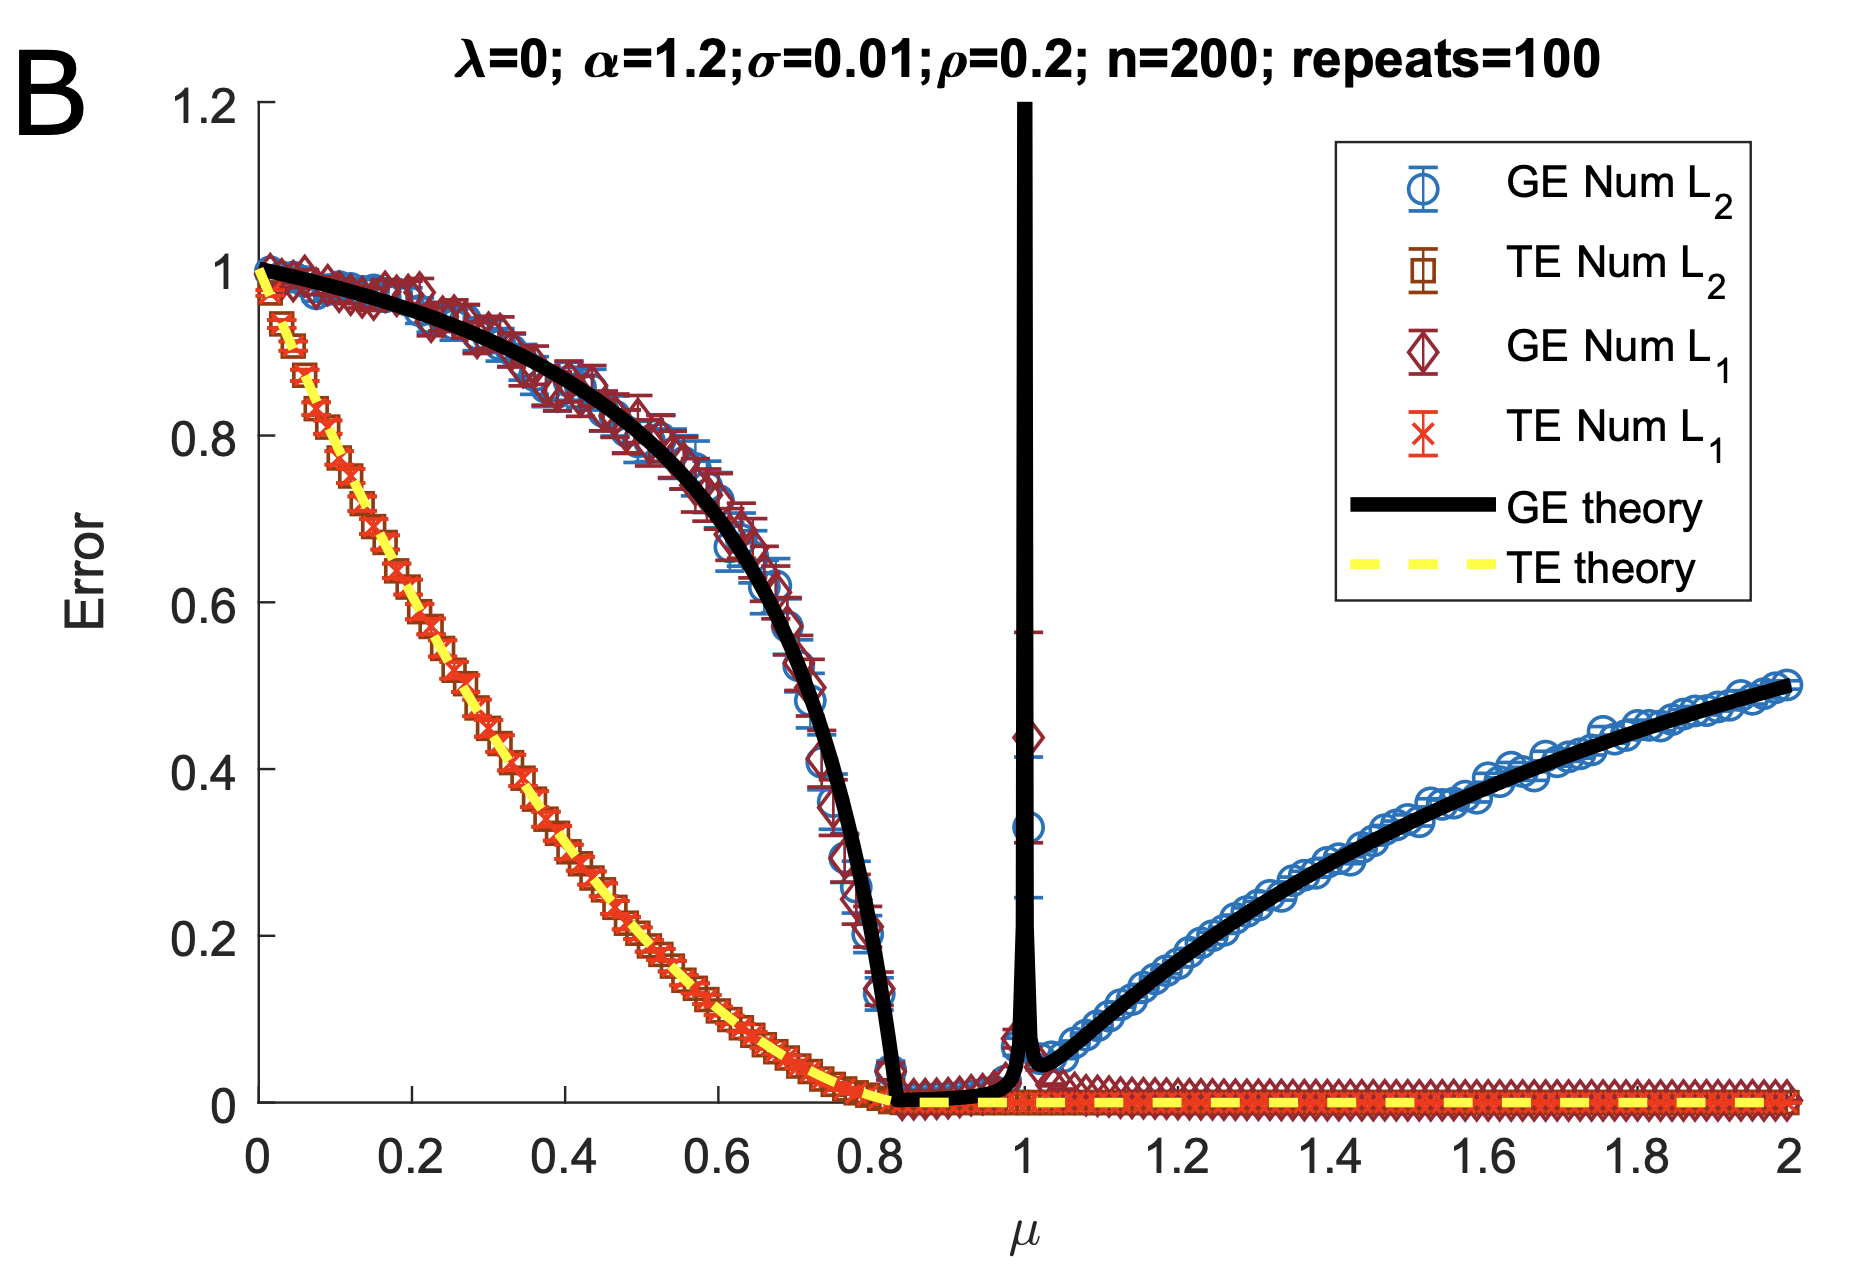
\includegraphics[width=0.8\linewidth]{part-4-images/mispar.png}

\vspace{-0.2cm}
{\scriptsize Source: \citep{mitra2019understanding}}
\end{center}

\end{column}
\end{columns}
\end{frame}
\begin{frame}{Models of double descent: Random feature models}
In random feature regression, the number of random features controls the model capacity, and can be tuned independently from the data.

Exact asymptotic results in high dimensions exist in many settings, including:
\begin{itemize}
    \item Unstructured random features~\citep{mei2019generalization}
    \item NTK-structured random features~\citep{adlam2020neural}
    \item Random Fourier features~\citep{liao2020random}
\end{itemize}
\begin{columns}
\begin{column}{0.5\linewidth}
\begin{center}
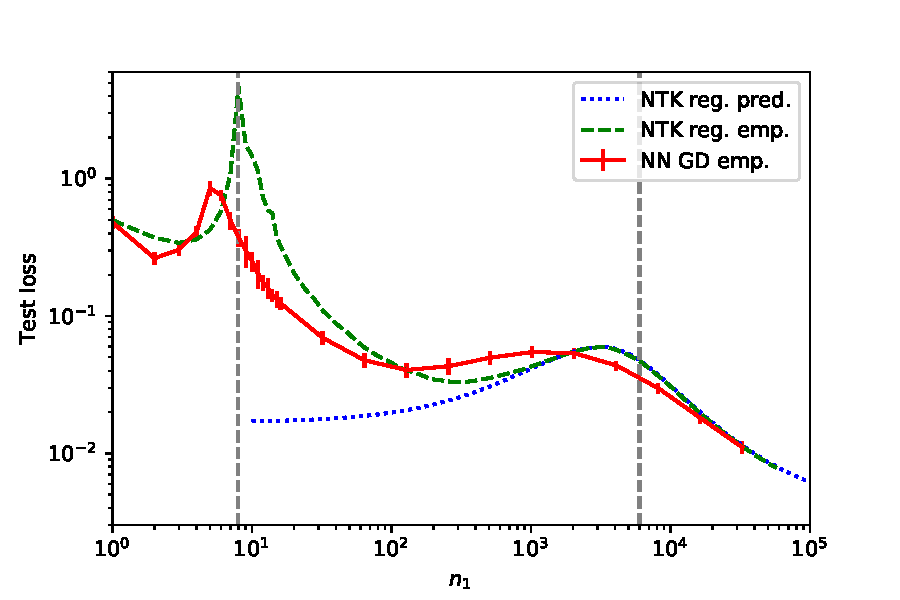
\includegraphics[width=0.75\linewidth]{part-4-images/gd_v2.pdf}

\vspace{-0.2cm}
{\scriptsize Source: \citep{adlam2020neural}}
\end{center}

\end{column}
\begin{column}{0.5\linewidth}
\begin{center}
% \vspace{-0.5cm}
\hspace{-1cm}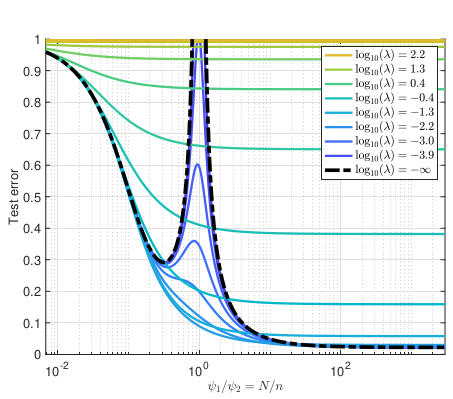
\includegraphics[width=0.6\linewidth]{part-1-images/mei-montanari-double-descent.png}

\vspace{-0.2cm}
\hspace{-1cm}
{\scriptsize Source: \citep{mei2019generalization}}
\end{center}

\end{column}
\end{columns}
\end{frame}
\section{Random feature models}
\begin{frame}[t]{Random feature regression: definition}
\emph{Random feature regression} is just linear regression on a transformed feature matrix, $\FF = f(\tfrac{1}{\sqrt{d}}\WW\XX) \in \mathbb{R}^{m \times n}$, where $\WW\in\mathbb{R}^{m\times d}$, $\WW_{ij}\sim \mathcal{N}(0,1)$.
\begin{itemize}
    \item Model given by $\bbeta^\top \FF$ (instead of $\bbeta^\top \XX$) --- variable capacity ($m$ vs $d$ parameters)
    \item $f(\cdot)$ is a nonlinear activation function, acting elementwise
    \item $\FF$ is equivalent to first post-activation layer of a NN at init
\end{itemize}
\pause
For targets $\YY\in\mathbb{R}^{1\times n}$, the ridge-regularized loss is, 
$$L(\bbeta; \XX) = \|\YY - \tfrac{1}{\sqrt{m}}\bbeta^\top \FF\|_2^2 + \lambda \|\bbeta\|_2^2\,,$$
and the optimal regression coefficients $\hat{\bbeta}$ are given by,
$$\hat{\bbeta} = \tfrac{1}{\sqrt{m}}\YY(\KK + \lambda \II_n)^{-1}\FF^\top\,,\quad \KK = \tfrac{1}{m}\FF^\top \FF\,.$$
\pause
Note that $\QQ \equiv (\KK + \lambda \II_n)^{-1}$ is the \emph{resolvent} of the kernel matrix $\KK$.
\end{frame}
\begin{frame}[t]{Random feature regression: training error}
Training error is determined by the resolvent matrix $\QQ\equiv (\KK + \lambda \II_n)^{-1}$:
\begin{align*}
E_{\text{train}}(\lambda) &=  \tfrac{1}{n}\|\YY - \tfrac{1}{\sqrt{m}}{\hat{\bbeta}}^\top \FF\|_2^2\\
&= \tfrac{1}{n}\|\YY-\tfrac{1}{m}\YY \QQ \FF^\top\FF\|_2^2\\
&= \tfrac{1}{n}\|\YY-\YY \QQ \KK\|_2^2\\
&= \tfrac{1}{n}\|\YY(\II_n-\QQ \KK)\|_2^2\\
&= \lambda^2\tfrac{1}{n}\|\YY\QQ\|_2^2\,,
% &= \tfrac{1}{n}(Y-\tfrac{1}{m}Y Q F^TF)(Y-\tfrac{1}{m}Y Q F^\top F)^\top\\
% &= \tfrac{1}{n}(Y-Y Q K)(Y-Y Q K)^\top\\
% &= \tfrac{1}{n}Y (I_n-Q K)^2 Y^\top\\
% &= \lambda^2 \tfrac{1}{n} Y Q^2 Y^\top\,.
\end{align*}
where we used that $\II_n - \QQ \KK = \II_n - \QQ (\QQ^{-1} - \lambda \II_n) =  \II_n -  (\II_n - \lambda \QQ) = \lambda \QQ$.
\pause

So we see that the training error measures the alignment between the resolvent and the label vector.

What about the test error?
% \begin{align*}
%     E_{\text{train}}(\lambda) &= \tfrac{1}{n}\text{tr}[(I_n-Q K)^\top Y^\top Y (I_n-Q K)]\\
%     &= \lambda^2 \tfrac{1}{n}\text{tr}[Y^\top Y Q^2]\\
%     &= -\lambda^2 \tfrac{\partial}{\partial \lambda}\tfrac{1}{n}\text{tr}[Y^\top Y Q]\,,
% \end{align*}
% so it suffices to understand $\tfrac{1}{n}\text{tr}[Y^\top Y Q]$, i.e. the projection of the resolvent into the label vector.
\end{frame}
\begin{frame}[t]{Aside: Generalized cross validation (GCV)}
A model's performance on the training set, or subsets thereof, can be useful for estimating its performance on the test set.
\begin{itemize}
    \item Leave-one-out cross validation (LOOCV)\\
$$E_{LOOCV}(\lambda) = \tfrac{1}{n}\|\YY\QQ\cdot\text{diag}(\QQ)^{-1}\|_2^2 $$
    \item Generalized cross validation (GCV)\\
    $$E_{GCV}(\lambda) = \tfrac{1}{n}\|\YY\QQ\|_2^2/(\tfrac{1}{n}\text{tr}(\QQ))^2$$
\end{itemize}
\pause

In certain high-dimensional limits, $E_{GCV}(\lambda) = E_{LOOCV}(\lambda) = E_{\text{test}}(\lambda)$:
\begin{itemize}
    \item Ridge regression~\citep{hastie2019surprises}
    \item Kernel ridge regression~\citep{jacot2020kernel}
    \item Random feature regression~\citep{adlam2020neural}
\end{itemize}
\end{frame}
\begin{frame}[t]{Random feature regression: high-dimensional asymptotics}
To develop an analytical model of double descent, we study the high-dimensional asymptotics:
$$ m,d,n \to \infty\,\quad \text{such that}\quad \phi \equiv \tfrac{d}{n}\;, \psi \equiv \tfrac{d}{m}\quad \text{are constant.}$$
\pause
In this limit, only \emph{linear} functions of the data can be learned.
\begin{itemize}
    \item Intuition: only enough constraints to disambiguate linear combinations of features.
    \item Nonlinear target function behaves like linear function plus noise%: $Y = y(X) \to \tfrac{1}{\sqrt{d}}{\bbeta^*}^\top X + \varepsilon$.
\end{itemize}
\pause
Therefore it suffices to consider labels given by
$$\YY = \tfrac{1}{\sqrt{d}}{\bbeta^*}^\top \XX + \bm{\varepsilon}\,,\quad \varepsilon_i \sim \mathcal{N}(0,\sigma_{\varepsilon}^2)\,.$$
\pause
For simplicity, we focus on the specific setting in which,
$$X_{ij}\sim \mathcal{N}(0,1)\quad \text{and}\quad{\bbeta^*} \sim \mathcal{N}(0,I_d)\,.$$
\end{frame}
\begin{frame}[t]{Random feature regression: test error}
In the high-dimensional asymptotic setup from above, the random feature test error can be written as,
\begin{align*}
    E_{\text{test}}(\lambda) &= E_{\text{GCV}}(\lambda)\\
    &= \lim_{n\to\infty} \tfrac{1}{n}\|\YY\QQ\|_2^2/(\tfrac{1}{n}\text{tr}(\QQ))^2\\
    &= \lim_{n\to\infty}\tfrac{1}{n} \|(\tfrac{1}{\sqrt{d}}{\bbeta^*}^\top \XX + \bm{\varepsilon})\QQ\|_2^2/(\tfrac{1}{n}\text{tr}(\QQ))^2\\
    &= \lim_{n\to\infty}\tfrac{1}{n} \text{tr}[(\sigma_{\varepsilon}^2 \II_n + \tfrac{1}{d}\XX^\top \XX)\QQ^2]/(\tfrac{1}{n}\text{tr}(\QQ))^2\\
    &\equiv -\frac{\sigma_{\varepsilon}^2 \tau_1'(\lambda) + \tau_2'(\lambda)}{\tau_1(\lambda)^2}\,,
\end{align*}
where we used that $\tfrac{\partial}{\partial \lambda} \QQ = -\QQ^2$, and we defined
$$ \tau_1 = \lim_{n\to\infty} \tfrac{1}{n}\text{tr}(\QQ)\,\quad \text{and} \quad \tau_2 = \lim_{n\to\infty} \tfrac{1}{n}\text{tr}(\tfrac{1}{d}\XX^\top \XX \QQ)\,.$$
\end{frame}
\begin{frame}{Computing the asymptotic test error}
To compute the test error, we need:% the Stieltjes transform of $K$, $\tau_1$, and one additional generalized trace object, $\tau_2$:
$$ \tau_1 = \lim_{n\to\infty} \tfrac{1}{n}\text{tr}(\KK+\lambda \II_n)^{-1}\,\quad \text{and} \quad \tau_2 = \lim_{n\to\infty} \tfrac{1}{n}\text{tr}(\tfrac{1}{d}\XX^\top \XX (\KK+\lambda \II_n)^{-1})\,.$$
\pause
Recalling the definition of $\KK$,
$$ \KK = \tfrac{1}{m}\FF^\top \FF\,,\quad \FF = f(\tfrac{1}{\sqrt{d}}\WW\XX)\,,$$
it is evident that the entries of $\FF$ are nonlinearly dependent. 
% \pause
\begin{itemize}
    \item Cannot simply utilize standard results for Wishart matrices
    \item Stieltjes transform is insufficient for $\tau_2$%: need information about eigenvector overlaps for $\tau_2$
\end{itemize}
\pause
These technical challenges can be overcome with two tricks:
\begin{itemize}
    \item[1.] Constructing an equivalent Gaussian linearized model
    \item[2.] Analyzing a suitably augmented resolvent
\end{itemize}
\end{frame}
\begin{frame}[t]{Computing the asymptotic test error: Gaussian equivalents}
The nonlinear dependencies in $\FF = f(\tfrac{1}{\sqrt{d}}\WW\XX)$ complicate the analysis.

Can we identify a simpler matrix in the same universality class?
\pause
\\

There exist constants $c_1$ and $c_2$ such that
$$\FF \cong \FF_\text{lin} \equiv c_1 \tfrac{1}{\sqrt{d}}\WW\XX + c_2 \bm{\Theta}\,,\quad \Theta_{ij}\sim\mathcal{N}(0,1)\,,$$
where $\FF \cong \FF_\text{lin}$ indicates the two matrices share all statistics relevant for computing the test error:
\begin{align*}
    \tau_1 &= \lim_{n\to\infty} \tfrac{1}{n}\text{tr}(\tfrac{1}{m}\FF^\top \FF+\lambda \II_n)^{-1} = \lim_{n\to\infty} \tfrac{1}{n}\text{tr}(\tfrac{1}{m}\FF_{\text{lin}}^\top \FF_{\text{lin}}+\lambda \II_n)^{-1}\\
    \tau_2 &= \lim_{n\to\infty} \tfrac{1}{n}\text{tr}(\tfrac{1}{d}\XX^\top \XX (\tfrac{1}{m}\FF^\top \FF+\lambda \II_n)^{-1}) = \lim_{n\to\infty} \tfrac{1}{n}\text{tr}(\tfrac{1}{d}\XX^\top \XX (\tfrac{1}{m}\FF_{\text{lin}}^\top \FF_{\text{lin}}+\lambda \II_n)^{-1})
\end{align*}
\pause

How can we compute these traces? Need to augment the resolvent.
\end{frame}
\begin{frame}[t]{Computing the asymptotic test error: resolvent method}
Recall from Part 2 that the resolvent method identifies consistency relations between suitably chosen submatrices of the resolvent.

Here we can undertake a similar analysis as in Part 2, but now on an augmented matrix,
$$ \HH = \begin{bmatrix}
    \lambda \II_n        &    \frac{1}{\sqrt{m}}\FF_{\text{lin}}^\top  \\
    \frac{1}{\sqrt{m}}\FF_{\text{lin}}  &   -\II_m
    \end{bmatrix}\,,
$$
which encodes the resolvent through $\QQ = (\KK + \lambda \II_n)^{-1} = [\HH^{-1}]_{1:n,1:n}$.
\pause

To derive consistency relations, we consider two submatrices: $\HH^{(1)}$ (leaving out row/column $1$), and $\HH^{(n+1)}$ (leaving out row/column $n+1$).

As before, we use the Sherman-Morrison formula to compute $[\HH^{(1)}]^{-1}$ and $[\HH^{(n+1)}]^{-1}$, and relate them to $\QQ$ and rows/columns of $\FF_\text{lin}$.

Straightforward concentration arguments eventually lead to coupled self-consistent equations for $\tau_1$ and $\tau_2$~\citep{adlam2019random}.
\end{frame}

\begin{frame}[t]{Computing the asymptotic test error: free probability}
An alternative augmentation of the resolvent completely linearizes the dependence on the random matrices:
$$  \MM = \begin{bmatrix}
        \lambda \II_n & \tfrac{c_2}{m}\bm{\Theta}^\top & \tfrac{c_1}{\sqrt{d} m} \XX^\top & 0 \\
        c_2 \bm{\Theta} & -\II_m & 0 & \tfrac{c_1}{\sqrt{d}} \WW \\
        0 & \WW^\top & -\II_d & 0 \\
        \XX & 0 & 0 & -\II_d
        \end{bmatrix}\,,
$$
where the Schur complement formula now gives,
$$\tau_1 = \lim_{n\to\infty} \tfrac{1}{n}\text{tr} ([\MM^{-1}]_{1,1})\,,\quad\text{and}\quad \tau_2 = \lim_{n\to\infty} \tfrac{1}{n}\text{tr}( [\MM^{-1}]_{4,3})\,.$$

The asymptotic blockwise traces $\text{tr}([\MM^{-1}]_{a,b})$ can themselves be computed using free probability~\citep{adlam2020neural}.
\end{frame}

\begin{frame}[t]{Computing the asymptotic test error: free probability}
$\MM$ is linear in the random matrices $\XX$, $\WW$, and $\bm{\Theta}$:

\small 
\begin{align*}
\MM &= \begin{bmatrix}
\lambda \II_n&0&0&0\\
0&-\II_m&0&0\\
0&0&-\II_d&0\\
0&0&0&-\II_d
\end{bmatrix} 
+ 
\begin{bmatrix}
0&0&\tfrac{c_1}{\sqrt{d} m} \XX^\top&0\\
0&0&0&0\\
0&0&0&0\\
\XX&0&0&0
\end{bmatrix} +
\begin{bmatrix}
0&0&0&0\\
0&0&0&\tfrac{c_1}{\sqrt{d}} \WW\\
0&\WW^\top&0&0\\
0&0&0&0
\end{bmatrix}
+
\begin{bmatrix}
0&\tfrac{c_2}{m}\bm{\Theta}^\top&0&0\\
 c_2 \bm{\Theta}&0&0&0\\
0&0&0&0\\
0&0&0&0
\end{bmatrix}
\end{align*}

Can we compute the blockwise traces with free probability via the $R$-transform?
\pause

Not naively: the additive terms are independent, but not free over $\mathbb{C}$.

However, they are free over $M_4(\mathbb{C})$, and there exists a suitable \emph{operator-valued} generalization of the $R$-transform that enables the necessary computations~\citep{mingo2017free}.

\end{frame}
\begin{frame}[t]{Asymptotic test error}
\begin{alertblock}{Theorem}
Let $\eta = \mathbb{E}[f(g)^2]$ and $\zeta = (\mathbb{E}[g f(g)])^2$ for $g\sim \mathcal{N}(0,1)$. Then, the asymptotic traces $\tau_1(\lambda)$ and $\tau_2(\lambda)$ are given by solutions to the polynomial system,
\begin{equation*}
  \zeta  \tau_1 \tau_2
   \left(1-\lambda \tau_1\right) = \phi/\psi\left(\zeta  \tau_1 \tau_2 + \phi(\tau_2 -\tau_1) \right) = \left(\tau_1-\tau_2\right) \phi  \left((\eta-\zeta)\tau_1+\zeta \tau_2\right)\,,
\end{equation*}
and, $E_{\text{train}} = -\lambda^2(\sigma_\varepsilon^2 \tau_1' + \tau_2')$ and $E_{\text{test}} = -(\sigma_\varepsilon^2 \tau_1' + \tau_2')/\tau_1^2$.
\end{alertblock}
\begin{center}
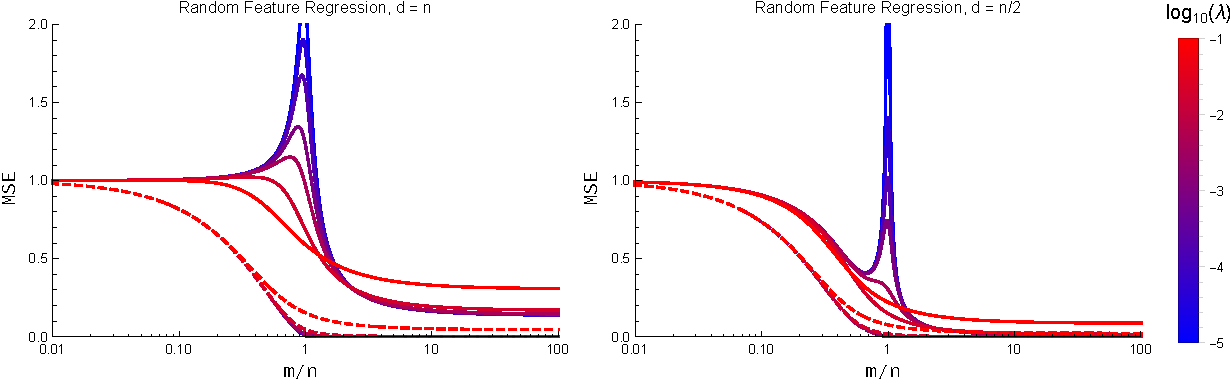
\includegraphics[width=0.9\linewidth]{part-4-images/RF_plots.pdf}
\end{center}
\end{frame}


\appendix



\begin{frame}[allowframebreaks]{References}

  \bibliographystyle{plainnat}
  {\scriptsize\bibliography{references}}

\end{frame}

\end{document}


